\section{Related work}
\label{sec:related_work}
This Section addresses existing contributions by examining similar experiments conducted, and existing standards in the I4.0 domain. 
In total, 4 papers are investigated.
\\ \\
Article \cite{Lasi2014} summarizes the evolution into the industry 4.0 system, and describes the fundamental concepts and goals for I4.0 systems. By localizing responsibilities throughout the system, it becomes possible to adapt faster, enabling quicker decision-making.
Encapsulating responsibilities to individual parts of the system, increases overall system interoperability and resource efficiency which allows the choice of different software for individual system parts. 
In principle, this should also increase modifiability and deployability, since each part of the system works independently and any updates or changes would only affect the singular part. 

By following these industry 4.0 principles and concepts, integration becomes possible and the production can make use of value-creation networks, which should allow for considerable optimization of processes and possibly gain insight into new aspects of revenue. With a dynamic production network, data can be collected throughout the whole product life cycle.



In \cite{torben21} a state-of-the-art production system developed for I4.0 systems has been proposed. The production system in the study focuses particularly on flexibility and adaptability in the production system and proposes a model to fulfill these quality attributes. The production system is built with a Microservice architecture, as the different subsystems are abstracted away by being dockerized. This causes the system to be adaptable and flexible, as small changes to the micro-services, in case the requirements change, can easily be deployed.  The subsystems then communicate through a message bus. The production line itself is built with a four-cell system, controlled by PLCs, that can function in multiple complex processes.
\\ \\
In \cite{torben20pilot} a pilot study of the interoperability quality attribute in a minimum viable product (MVP) of producing a drone has been analyzed. The setting of creating the drone is a modern state-of-the-art I4.0 laboratory, where multiple communication protocols and other assets, e.g. the cells in the production line, are required to work together to produce the product. Through an analysis of these assets communicating, it is concluded that the interoperability in I4.0 systems is still immature. This is because of a lack of various requirements of interoperability from the different assets, such as a lack of good documentation, missing external interfaces, and other communication technologies. The reason for this could be an apparent lack of understanding of the necessity of asset interoperability in an I4.0 context.


For insight into how an I4.0 system could be applied to actual production, article \cite{Liu2022} analyzes several other scientific articles on the topic. The article concludes with the creation of a prototype, with the purpose of testing the system architecture. The architecture for the prototype is based on a comprehensive literature review and gap analysis of industry 4.0 platforms.

\begin{figure*}[!ht]
    \centering
    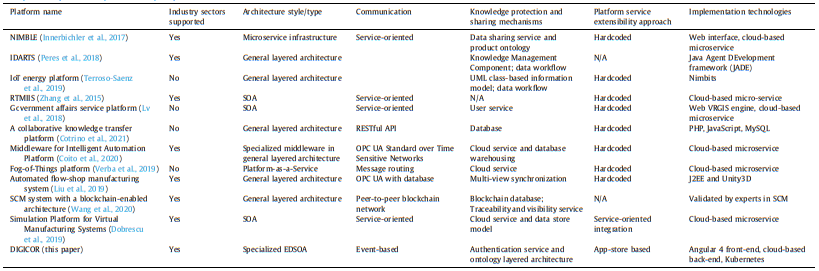
\includegraphics[scale=0.85]{Images/ArticleReviewRotate.png}
    \caption{Overview of system-architectures used for I4.0}
    \label{figure:1}
\end{figure*}


As seen in figure \ref{figure:1} from article \cite{Liu2022} the majority of the literature related to I4.0 uses different architectures, and an industry standard has not been formed. The article concludes that diverse quality attribute prioritization drives the different system architectures in different directions. After reviewing several of the different architectures, the authors decided that their system prototype's requirements aligned with either a micro-services or event-based architecture. In the end, when comparing the two, the event-based system allowed for higher performance, while keeping the interoperability aspect. The micro-service architecture added additional layers of complexity and fell behind in performance. In the end, the event-based architecture was decided for the prototype, as it had many of the perks of a micro-services architecture, while still maintaining a high performance.

